%!TeX root=main.tex

\section{Condicionales}

%\subsection*{Uso de \maximain{if}}
La orden condicional \maximain{if} es una sentencia
que comprueba si se verifica una condición,
si es verdadera ejecutará la expresión a continuación
del \maximain{then} y si es falsa ejecutará la
expresión después de \maximain{else}. La última es
opcional.

\begin{center}
	\maximain{if} condición \maximain{then} expr1
\end{center}
\begin{center}
	\maximain{if} condición \maximain{then} expr1
	\maximain{else} expr2
\end{center}

\begin{maximai}
if sin(4) < 9/10 and 2^2=4 then 1 else -1;
\end{maximai}
\begin{maximao}
1
\end{maximao}

\begin{maximai}
if sin(4) < -9/10 or 2^2=5 then 1 else -1;
\end{maximai}
\begin{maximao}
-1
\end{maximao}

\begin{maximai}
if sin(4)>cos(5) then 1;
\end{maximai}
\begin{maximao}
\mathbf{false}
\end{maximao}

\begin{maximai}
if sin(4)<cos(5) then 1;
\end{maximai}
\begin{maximao}
1
\end{maximao}

La sentencia condicional \maximain{if} es necesaria para definir
funciones a trozos. Por ejemplo para definir la función
\begin{equation*}
	F(x)=\left\{ \begin{array}{cl}
		0 & \text{ si } x<0, \\
		x^2 & \text{ si } x\geq0. \\
	\end{array}\right.
\end{equation*}

\begin{maximai}
F(x):=if x<0 then 0 else x^2$
\end{maximai}

\begin{maximai}
F(-1); F(0); F(3);
\end{maximai}
\begin{maximao}
0
\end{maximao}
\begin{maximaoo}
0
\end{maximaoo}
\begin{maximaoo}
9
\end{maximaoo}

%c F(x):=if x<0 then 0 else x^2$
%c plot2d(F(x),[x,-1,1],[y,-1,1], [pdf_file, "./plot_F.pdf"])$
%x
\begin{maximai}
	wxplot2d(F(x),[x,-1,1],[y,-1,1])$
\end{maximai}\begin{maximat}
	\begin{center}
		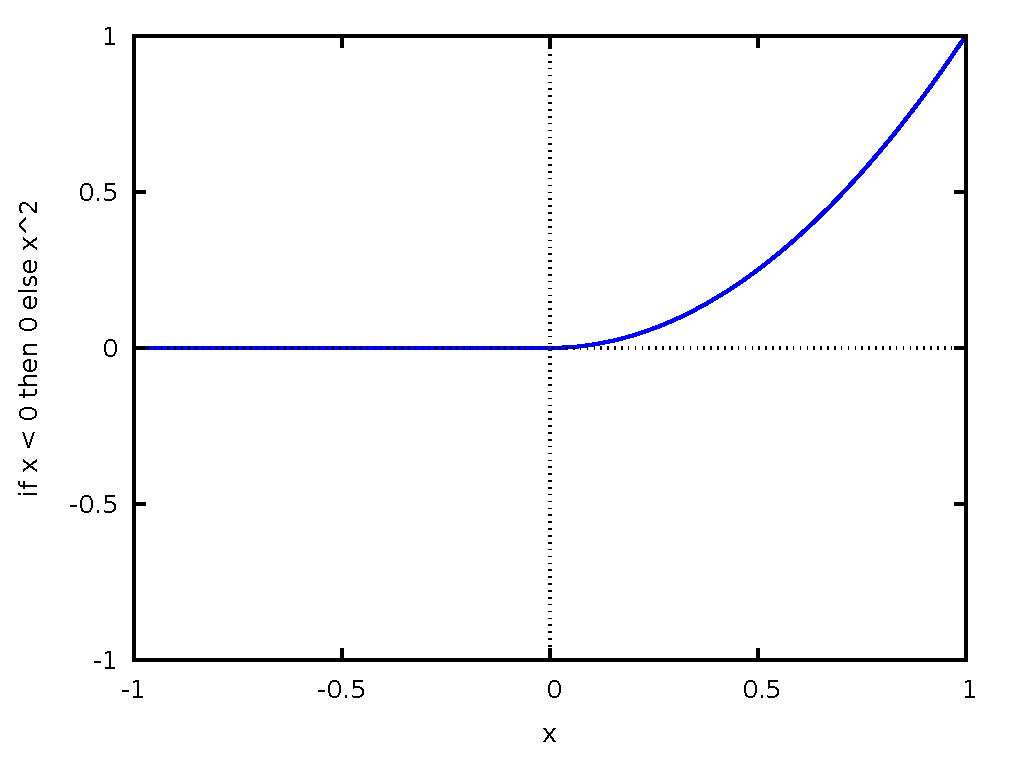
\includegraphics[scale=.5]{plot_F.pdf}
	\end{center}
\end{maximat}

A continaución definamos una función que está definida por
partes en tres intervalos diferentes.
\begin{equation*}
	G(x)=\left\{ \begin{array}{cl}
		0 & \text{ si } x<0, \\
		1 & \text{ si } 0\leq x\leq 1, \\
		x^2 & \text{ si } x>1. \\
	\end{array}\right.
\end{equation*}

\begin{maximai}
G(x):=if x<0 then 0 else (if x>1 then x^2 else 1)$
\end{maximai}

\begin{maximai}
G(.5);
\end{maximai}
\begin{maximao}
1
\end{maximao}

%c G(x):=if x<0 then 0 else (if x>1 then x^2 else 1)$
%c plot2d(G(x),[x,-1,3],[y,-1,9], [pdf_file, "./plot_G.pdf"])$
%x
\begin{maximai}
	wxplot2d(G(x),[x,-1,3],[y,-1,9])$
\end{maximai}\begin{maximat}
	\begin{center}
		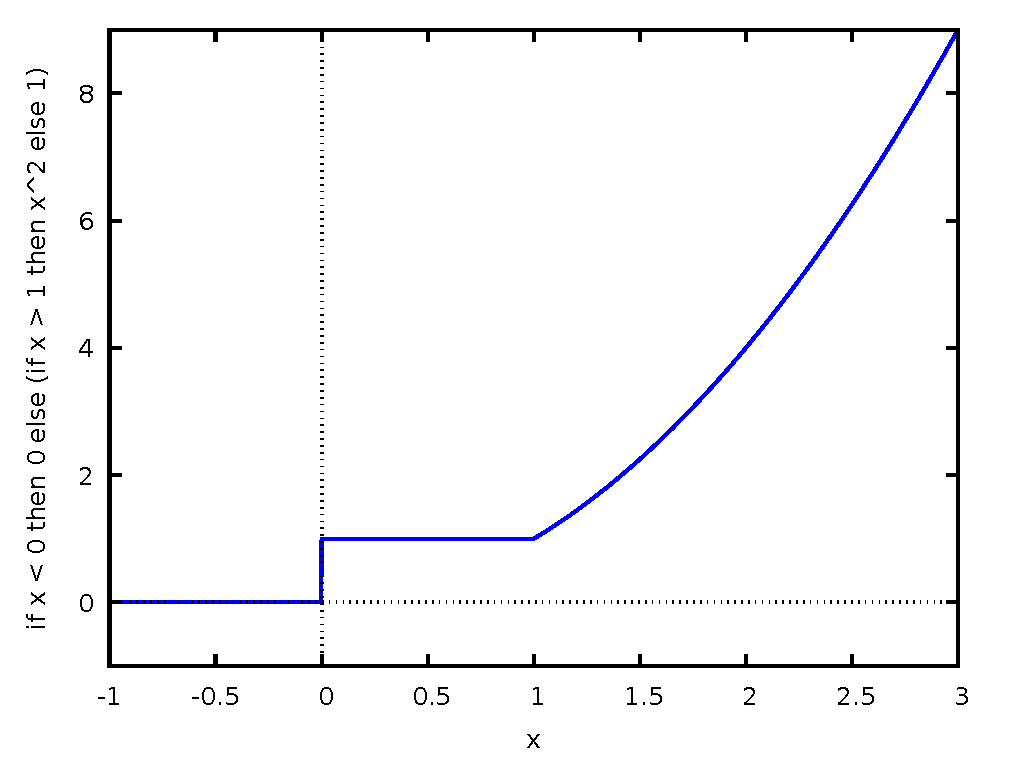
\includegraphics[scale=.5]{plot_G.pdf}
	\end{center}
\end{maximat}

En el caso anterior se dice que los \maximain{if} están anidados.
Ya que este uso es muy frecuente en programación, maxima incorpora
una palabra especial llamada \maximain{elseif}.
De este modo la función anterior se podría definir más facilmente.

\begin{maximai}
G(x):=if x<0 then 0 elseif x>1 then x^2 else 1$
\end{maximai}

%c G(x):=if x<0 then 0 elseif x>1 then x^2 else 1$
%c plot2d(G(x),[x,-1,3],[y,-1,9], [pdf_file, "./plot_G2.pdf"])$
%x
\begin{maximai}
	wxplot2d(G(x),[x,-1,3],[y,-1,9])$
\end{maximai}\begin{maximat}
	\begin{center}
		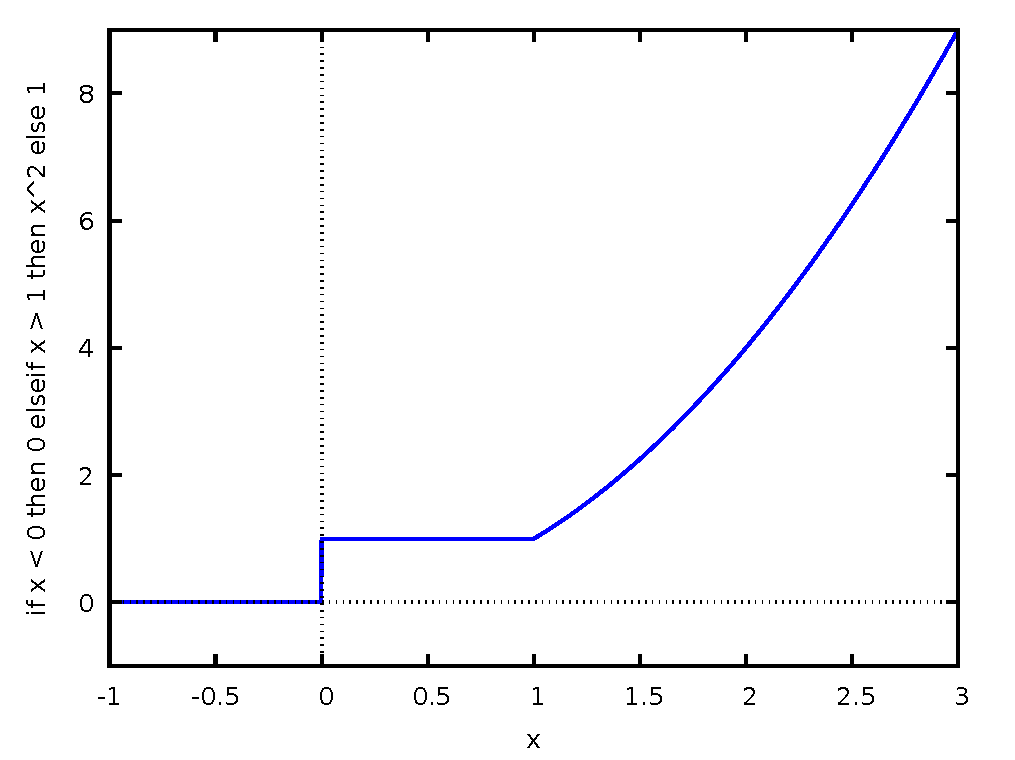
\includegraphics[scale=.5]{plot_G2.pdf}
	\end{center}
\end{maximat}

A continuación veamos varios ejemplos de funciones que usan
condicionales para ser definidas.

La función \maximain{max3} toma tres argumentos y devuelve
el elemento mayor.

\begin{maximai}
	max3(x,y,z):= if (x>=y and x>=z) then x
\end{maximai}\begin{maximal}
	elseif (y>=x and y>=z) then y else z$
\end{maximal}

\begin{maximai}
	max3(-1,5,3);
\end{maximai}
\begin{maximao}
	5
\end{maximao}

La función \maximain{signo} devuelve el signo de un número.

\begin{maximai}
signo(x):=if x>0 then 1 elseif x<0 then -1 else 0$
\end{maximai}

\begin{maximai}
[signo(1),signo(-3),signo(0)];
\end{maximai}
\begin{maximao}
\left[ 1 , -1 , 0 \right] 
\end{maximao}
